% ============================================================================
% TOPIC 18B: DIFFUSION-CONTROLLED REACTIONS
% ============================================================================

\section{Topic 18B: Diffusion-Controlled Reactions}

% ===========================================================================
% Slide 21: Topic 18B Overview
% ===========================================================================
\begin{frame}{Topic 18B: Diffusion-Controlled Reactions}

\textbf{Moving from Gas to Liquid Phase}

\vspace{0.3cm}

\begin{columns}[T]
\column{0.5\textwidth}
\textbf{Gas Phase:}
\begin{itemize}
\item Molecules fly freely
\item Single collisions
\item Low density ($\sim 10^{25}$ m$^{-3}$)
\item Long mean free path ($\sim$ 100 nm)
\item Collision frequency $\sim 10^{10}$ s$^{-1}$
\end{itemize}

\vspace{0.2cm}
\textbf{Liquid Phase:}
\begin{itemize}
\item Molecules are crowded
\item \alert{Cage Effect} - trapped by solvent
\item High density ($\sim 10^{28}$ m$^{-3}$)
\item Short mean free path ($\sim$ 0.3 nm)
\item \alert{Diffusion} limits encounter rate
\end{itemize}

\column{0.5\textwidth}
\centering
\textbf{Solvent Cage Effect:}

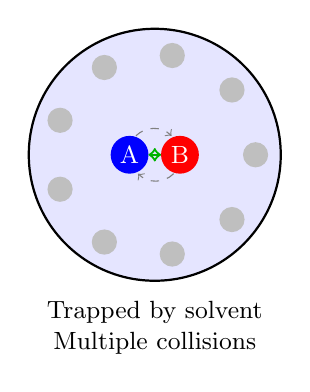
\begin{tikzpicture}[scale=0.8]
    % Cage effect diagram
    \draw[fill=blue!10, thick] (0,0) circle (2cm);

    % Solvent molecules forming cage
    \foreach \angle in {0,40,80,120,160,200,240,280,320}
        \fill[gray!50] ({1.6*cos(\angle)}, {1.6*sin(\angle)}) circle (0.2cm);

    % Reactant molecules inside cage
    \fill[blue] (-0.4,0) circle (0.3cm) node[white] {\small A};
    \fill[red] (0.4,0) circle (0.3cm) node[white] {\small B};

    % Multiple collision arrows
    \draw[<->, thick, green!70!black] (-0.1,0) -- (0.1,0);
    \draw[->, dashed, gray] (-0.3,0.3) arc (135:45:0.4);
    \draw[->, dashed, gray] (0.3,-0.3) arc (-45:-135:0.4);

    \node at (0,-2.5) {\small Trapped by solvent};
    \node at (0,-3) {\small Multiple collisions};
\end{tikzpicture}
\end{columns}

\end{frame}

% ===========================================================================
% Slide: Encounter Pairs
% ===========================================================================
\begin{frame}{The Concept of Encounter Pairs}

\begin{block}{Encounter Pair}
When two reactants A and B meet in solution, they are temporarily trapped in a solvent cage and undergo multiple collisions before separating.
\end{block}

\vspace{0.15cm}

\begin{columns}[T]
\column{0.5\textwidth}
\textbf{Key Differences from Gas Phase:}
\begin{itemize}
\item \textbf{Gas:} One collision per encounter
\item \textbf{Liquid:} $\sim 10^2 - 10^3$ collisions per encounter
\item Collision frequency within cage: $\sim 10^{13}$ s$^{-1}$
\item Cage lifetime: $\sim 10^{-11}$ s
\item Effective "single" encounter
\end{itemize}

\column{0.5\textwidth}
\centering
\textbf{Encounter Dynamics:}

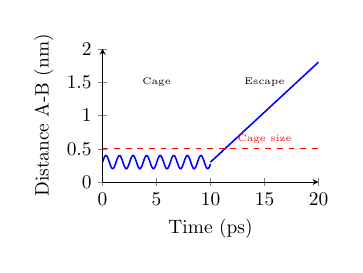
\begin{tikzpicture}[scale=0.7]
\begin{axis}[
    xlabel={Time (ps)},
    ylabel={Distance A-B (nm)},
    xmin=0, xmax=20,
    ymin=0, ymax=2,
    axis lines=left,
    width=5.5cm,
    height=4cm
]
% Oscillating distance representing cage dynamics
\addplot[blue, thick, domain=0:10, samples=100] {0.3 + 0.1*sin(deg(x*5))};
\addplot[blue, thick, domain=10:20, samples=50] {0.3 + (x-10)*0.15};
\draw[dashed, red] (axis cs:0,0.5) -- (axis cs:20,0.5);
\node[red] at (axis cs:15,0.65) {\tiny Cage size};
\node at (axis cs:5,1.5) {\tiny Cage};
\node at (axis cs:15,1.5) {\tiny Escape};
\end{axis}
\end{tikzpicture}
\end{columns}

\vspace{0.1cm}
\emphbox{For fast reactions: Rate limited by how quickly reactants find each other}

\end{frame}

% ===========================================================================
% Slide: Two Limiting Regimes
% ===========================================================================
\begin{frame}{Two Limiting Regimes}

\begin{columns}[T]
\column{0.5\textwidth}
\begin{block}{Diffusion-Controlled}
\textbf{Fast Reaction}
\begin{itemize}
\item $k_a \gg k_{-d}$ (reaction faster than separation)
\item Every encounter leads to reaction
\item Rate limited by \alert{transport} (diffusion)
\item Low activation energy ($E_a \approx E_{viscosity}$)
\item Examples: Radical recombination, H$^+$ + OH$^-$
\end{itemize}
\vspace{0.2cm}
\keyeq{k \approx k_d \sim 10^{10} \text{ M}^{-1}\text{s}^{-1}}
\end{block}

\column{0.5\textwidth}
\begin{block}{Activation-Controlled}
\textbf{Slow Reaction}
\begin{itemize}
\item $k_a \ll k_{-d}$ (separation faster than reaction)
\item Many encounters before reaction
\item Rate limited by \alert{energy barrier}
\item High activation energy
\item Behaves like gas-phase kinetics
\end{itemize}
\vspace{0.2cm}
\keyeq{k \propto e^{-E_a/RT}}
\end{block}
\end{columns}

\vspace{0.3cm}

\textbf{The Crossover:} Many reactions show intermediate behavior!

\end{frame}

% ===========================================================================
% Slide: Mechanism of Diffusion-Controlled Reactions Part 1
% ===========================================================================
\begin{frame}{Mechanism: The Two-Step Model (Part 1)}

\textbf{Reaction Scheme:}

\[ \ch{A + B <=>[ k_d ][ k_{-d} ] [AB] ->[ k_a ] P} \]

\vspace{0.3cm}

\textbf{Elementary Steps:}
\begin{enumerate}
\item \textbf{Diffusion together:} A + B $\xrightarrow{k_d}$ [AB]
\begin{itemize}
\item $k_d$: Diffusion rate constant
\item Formation of encounter pair
\item Limited by diffusion coefficient $D$
\end{itemize}

\item \textbf{Diffusion apart:} [AB] $\xrightarrow{k_{-d}}$ A + B
\begin{itemize}
\item $k_{-d}$: Separation rate constant
\item Breakup of encounter pair
\item Also diffusion-controlled
\end{itemize}

\item \textbf{Reaction:} [AB] $\xrightarrow{k_a}$ P
\begin{itemize}
\item $k_a$: Activation rate constant
\item Chemical transformation within cage
\item Depends on $E_a$
\end{itemize}
\end{enumerate}

\end{frame}

% ===========================================================================
% Slide: Mechanism Energy Diagram
% ===========================================================================
\begin{frame}{Mechanism: Energy Diagram}

\begin{columns}[T]
\column{0.5\textwidth}
\textbf{Free Energy Profile:}

\vspace{0.2cm}

\begin{itemize}
\item A + B $\to$ [AB]: Diffusion barrier (small)
\item [AB] $\to$ [AB]$^\ddagger$: Activation barrier
\item [AB]$^\ddagger$ $\to$ P: Reaction
\end{itemize}

\vspace{0.3cm}

The rate-limiting step depends on relative barrier heights!

\column{0.5\textwidth}
\centering
\textbf{Energy Diagram:}

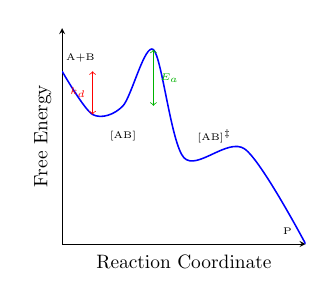
\begin{tikzpicture}[scale=0.7]
\begin{axis}[
    xlabel={Reaction Coordinate},
    ylabel={Free Energy},
    xmin=0, xmax=4,
    ymin=0, ymax=5,
    axis lines=left,
    xtick=\empty,
    ytick=\empty,
    width=6cm,
    height=5.5cm
]
% Energy profile
\addplot[blue, thick, smooth] coordinates {
    (0,4) (0.5,3) (1,3.2) (1.5,4.5) (2,2) (3,2.2) (4,0)
};
\node at (axis cs:0.3,4.3) {\tiny A+B};
\node at (axis cs:1,2.5) {\tiny [AB]};
\node at (axis cs:2.5,2.5) {\tiny [AB]$^\ddagger$};
\node at (axis cs:3.7,0.3) {\tiny P};

% Arrows
\draw[<->, red] (axis cs:0.5,3) -- (axis cs:0.5,4) node[midway, left] {\tiny $k_d$};
\draw[<->, green!70!black] (axis cs:1.5,3.2) -- (axis cs:1.5,4.5) node[midway, right] {\tiny $E_a$};
\end{axis}
\end{tikzpicture}
\end{columns}

\end{frame}

% ===========================================================================
% Slide: Steady-State Treatment Part 1
% ===========================================================================
\begin{frame}{Steady-State Treatment (Part 1)}

\textbf{Apply steady-state approximation to encounter pair [AB]:}

\[ \frac{d[\text{AB}]}{dt} = k_d[A][B] - k_{-d}[\text{AB}] - k_a[\text{AB}] = 0 \]

\vspace{0.3cm}

\textbf{Solve for [AB]:}
\[ [\text{AB}] = \frac{k_d[A][B]}{k_{-d} + k_a} \]

\vspace{0.3cm}

\textbf{Rate of product formation:}
\[ \text{Rate} = k_a[\text{AB}] = \frac{k_a k_d}{k_{-d} + k_a} [A][B] \]

\end{frame}

% ===========================================================================
% Slide: Steady-State Treatment Part 2
% ===========================================================================
\begin{frame}{Steady-State Treatment (Part 2)}

\textbf{Overall rate constant:}
\[ k_{eff} = \frac{k_a k_d}{k_{-d} + k_a} \]

\vspace{0.3cm}

\textbf{Rearrange to resistance form:}
\keyeq{\frac{1}{k_{eff}} = \frac{1}{k_d} + \frac{1}{K k_a}}

where $K = k_d/k_{-d}$ is the equilibrium constant for encounter pair formation.

\vspace{0.3cm}

\emphbox{Two resistances in series: diffusion and activation}

\vspace{0.3cm}

\textbf{Interpretation:} Like electrical resistances, the slower step dominates!

\end{frame}

% ===========================================================================
% Slide: Limiting Cases Derived
% ===========================================================================
\begin{frame}{Limiting Cases from the General Expression}

\textbf{General Result:}
\[ k_{eff} = \frac{k_a k_d}{k_{-d} + k_a} \]

\vspace{0.3cm}

\begin{columns}[T]
\column{0.5\textwidth}
\textbf{Case 1: Diffusion Control}

$k_a \gg k_{-d}$ (fast reaction)

\[ k_{eff} = \frac{k_a k_d}{k_a} = k_d \]

\begin{itemize}
\item Rate independent of $k_a$
\item Maximum possible rate
\item $k_{eff} \sim 10^{10}$ M$^{-1}$ s$^{-1}$
\item Weak temperature dependence
\item $E_a \approx E_{viscosity} \approx 10-20$ kJ/mol
\end{itemize}

\column{0.5\textwidth}
\textbf{Case 2: Activation Control}

$k_a \ll k_{-d}$ (slow reaction)

\[ k_{eff} = \frac{k_d}{k_{-d}} k_a = K k_a \]

\begin{itemize}
\item Rate proportional to $k_a$
\item Arrhenius behavior
\item Strong temperature dependence
\item $E_a$ = activation barrier
\item Same as gas-phase kinetics
\end{itemize}
\end{columns}

\vspace{0.3cm}

\textbf{Physical Interpretation:} In activation control, pairs form and break many times before reacting (equilibrium established).

\end{frame}

% ===========================================================================
% Slide: Fick's First Law
% ===========================================================================
\begin{frame}{Fick's First Law of Diffusion}

\textbf{Foundation of Diffusion Theory:}

\vspace{0.3cm}

\textbf{Fick's First Law} (steady-state):
\keyeq{J = -D \frac{\partial c}{\partial x}}

\vspace{0.3cm}

\textbf{Physical Interpretation:}
\begin{itemize}
\item $J$: Flux (mol m$^{-2}$ s$^{-1}$) - flow rate per unit area
\item $D$: Diffusion coefficient (m$^2$ s$^{-1}$)
\item $\frac{\partial c}{\partial x}$: Concentration gradient
\item Negative sign: Flow from high to low concentration
\end{itemize}

\vspace{0.3cm}

\textbf{Typical Values:} $D \sim 10^{-9}$ m$^2$ s$^{-1}$ in water (small molecules)

\end{frame}

% ===========================================================================
% Slide: Fick's Second Law
% ===========================================================================
\begin{frame}{Fick's Second Law of Diffusion}

\textbf{Fick's Second Law} (time-dependent):
\keyeq{\frac{\partial c}{\partial t} = D \frac{\partial^2 c}{\partial x^2}}

\vspace{0.3cm}

\textbf{Physical Interpretation:}
\begin{itemize}
\item Describes how concentration evolves in time
\item Parabolic partial differential equation (diffusion/heat equation)
\item In 3D: $\frac{\partial c}{\partial t} = D \nabla^2 c$
\item Solution gives $c(x,t)$ - concentration distribution
\end{itemize}

\vspace{0.3cm}

\emphbox{These laws form the mathematical foundation for Smoluchowski theory}

\end{frame}

% ===========================================================================
% Slide: Stokes-Einstein Relation Part 1
% ===========================================================================
\begin{frame}{Stokes-Einstein Relation (Part 1)}

\textbf{Connection between diffusion and molecular properties:}

\vspace{0.3cm}

For a spherical particle of radius $r$ moving through liquid of viscosity $\eta$:

\keyeq{D = \frac{k_B T}{6\pi \eta r}}

\vspace{0.3cm}

\textbf{Physical Basis:}
\begin{itemize}
\item Stokes drag force: $F = 6\pi \eta r v$
\item Einstein relation: $D = \mu k_B T$ where $\mu = 1/6\pi\eta r$
\item Connects microscopic (diffusion) to macroscopic (viscosity)
\end{itemize}

\vspace{0.3cm}

\textbf{Key Dependencies:}
\begin{itemize}
\item $D \propto T$ (faster at higher temperature)
\item $D \propto 1/\eta$ (slower in viscous media)
\item $D \propto 1/r$ (smaller molecules diffuse faster)
\end{itemize}

\end{frame}

% ===========================================================================
% Slide: Stokes-Einstein Relation Part 2
% ===========================================================================
\begin{frame}{Stokes-Einstein Relation (Part 2)}

\begin{columns}[T]
\column{0.5\textwidth}
\textbf{Typical Values at 25°C:}

\begin{table}
\small
\begin{tabular}{lcc}
\toprule
\textbf{Species} & $r$ (nm) & $D$ (10$^{-9}$ m$^2$/s) \\
\midrule
H$_2$O & 0.14 & 2.3 \\
Glycerol & 0.3 & 1.0 \\
Hemoglobin & 3.1 & 0.069 \\
\bottomrule
\end{tabular}
\end{table}

\column{0.5\textwidth}
\textbf{Viscosity of Water:}
\begin{itemize}
\item 25°C: $\eta = 0.89$ mPa$\cdot$s
\item 0°C: $\eta = 1.79$ mPa$\cdot$s
\item Strong T-dependence!
\end{itemize}

\vspace{0.3cm}

\textbf{Observation:}
\begin{itemize}
\item Larger molecules: smaller $D$
\item Size effect is dramatic (factor of 30!)
\end{itemize}
\end{columns}

\vspace{0.3cm}

\emphbox{Stokes-Einstein is remarkably accurate for molecules in solution}

\end{frame}

% ===========================================================================
% Slide: Smoluchowski Theory - Setup
% ===========================================================================
\begin{frame}{Smoluchowski Theory: Deriving $k_d$}

\textbf{Goal:} Calculate the rate constant for diffusion-controlled encounter.

\vspace{0.2cm}

\textbf{Model Assumptions:}
\begin{enumerate}
\item Molecule A is stationary at origin
\item B molecules diffuse toward A with diffusion coefficient $D = D_A + D_B$
\item Reaction occurs when B reaches distance $R^* = r_A + r_B$ (contact)
\item Steady-state concentration profile of B around A
\item B molecules are consumed at $r = R^*$ (perfect sink)
\end{enumerate}

\vspace{0.2cm}

\textbf{Boundary Conditions:}
\begin{itemize}
\item At $r = R^*$: $[B] = 0$ (instantaneous reaction)
\item As $r \to \infty$: $[B] = [B]_{bulk}$ (uniform far away)
\end{itemize}

\vspace{0.2cm}

\emphbox{Solve Fick's law in spherical coordinates with these boundary conditions}

\end{frame}

% ===========================================================================
% Slide: Smoluchowski Derivation
% ===========================================================================
\begin{frame}{Smoluchowski Derivation}

\textbf{Fick's First Law in spherical coordinates (steady-state):}
\[ J(r) = -D \frac{d[B]}{dr} \]

\textbf{Continuity equation (spherical):}
\[ \frac{1}{r^2} \frac{d}{dr}\left(r^2 J\right) = 0 \]

This gives: $r^2 J = \text{constant}$

\vspace{0.2cm}

\textbf{Solution with boundary conditions:}
\[ [B](r) = [B]_{bulk} \left(1 - \frac{R^*}{r}\right) \]

\textbf{Flux at contact surface:}
\[ J(R^*) = -D \left.\frac{d[B]}{dr}\right|_{r=R^*} = D \frac{[B]_{bulk}}{R^*} \]

\textbf{Total rate (flux × area):}
\[ \text{Rate} = 4\pi (R^*)^2 \cdot J(R^*) = 4\pi R^* D [B]_{bulk} \]

\end{frame}

% ===========================================================================
% Slide: Smoluchowski Result
% ===========================================================================
\begin{frame}{Smoluchowski Result for $k_d$}

\textbf{From flux calculation:}
\[ \text{Rate} = 4\pi R^* D [A][B] \]

\textbf{Compare with rate law:} Rate = $k_d[A][B]$

\vspace{0.2cm}

\keyeq{k_d = 4\pi R^* D N_A}

where $N_A$ converts to molar units.

\vspace{0.3cm}

\textbf{Using Stokes-Einstein:} $D = \frac{k_B T}{6\pi \eta r}$

For similar-sized molecules: $R^* \approx 2r$ and $D \approx \frac{k_B T}{6\pi \eta r}$

\keyeq{k_d \approx \frac{8RT}{3\eta}}

\vspace{0.2cm}

\textbf{Remarkable Result:}
\begin{itemize}
\item $k_d$ depends mainly on $T$ and $\eta$
\item Nearly independent of molecular size (cancellation!)
\item Universal diffusion limit for reactions in solution
\end{itemize}

\end{frame}

% ===========================================================================
% Slide: Numerical Estimate
% ===========================================================================
\begin{frame}{Numerical Estimate of Diffusion Limit}

\textbf{For water at 25°C:}

\textbf{Given:}
\begin{itemize}
\item $T = 298$ K
\item $\eta = 8.9 \times 10^{-4}$ Pa$\cdot$s
\item $R = 8.314$ J mol$^{-1}$ K$^{-1}$
\end{itemize}

\vspace{0.2cm}

\textbf{Calculation:}
\[ k_d = \frac{8RT}{3\eta} = \frac{8 \times 8.314 \times 298}{3 \times 8.9 \times 10^{-4}} \]

\[ k_d = \frac{19{,}830}{0.00267} = 7.4 \times 10^6 \text{ m}^3 \text{ mol}^{-1} \text{ s}^{-1} \]

\vspace{0.2cm}

\keyeq{k_d \approx 7 \times 10^9 \text{ dm}^3 \text{ mol}^{-1} \text{ s}^{-1} = 7 \times 10^9 \text{ M}^{-1} \text{ s}^{-1}}

\vspace{0.3cm}

\emphbox{This is the \textbf{diffusion limit}: Maximum possible rate in aqueous solution}

\textbf{Note:} If you measure $k > 10^{10}$ M$^{-1}$ s$^{-1}$, check for errors or special mechanisms (e.g., long-range forces, harpoon reactions).

\end{frame}

% ===========================================================================
% Slide: Temperature Dependence
% ===========================================================================
\begin{frame}{Temperature Dependence of Diffusion-Controlled Reactions}

\textbf{From Smoluchowski:} $k_d = \frac{8RT}{3\eta}$

\vspace{0.2cm}

\textbf{Temperature dependence comes from:}
\begin{enumerate}
\item Direct $T$ factor: $k_d \propto T$
\item Viscosity: $\eta(T)$ decreases with increasing $T$
\end{enumerate}

\vspace{0.2cm}

\textbf{Viscosity Temperature Dependence:}
\[ \eta(T) = \eta_0 e^{E_{\eta}/RT} \]

Typical values: $E_\eta \approx 10-20$ kJ/mol for liquids

\vspace{0.2cm}

\textbf{Combined effect:}
\[ k_d \propto \frac{T}{\eta(T)} \propto T e^{-E_{\eta}/RT} \]

Taking logarithm and differentiating:
\[ \frac{d \ln k_d}{d(1/T)} = -\frac{E_{\eta}}{R} + \frac{RT}{T} = -\frac{E_{\eta} - RT}{R} \]

\keyeq{E_{a,diff} \approx E_{\eta} - RT \approx E_{\eta} - 2.5 \text{ kJ/mol}}

\textbf{Typical:} $E_{a,diff} \sim 10-20$ kJ/mol (much smaller than chemical activation!)

\end{frame}

% ===========================================================================
% Slide: Comparison with Experimental Data
% ===========================================================================
\begin{frame}{Experimental Verification}

\textbf{Examples of Diffusion-Controlled Reactions:}

\vspace{0.2cm}

\begin{table}
\centering
\small
\begin{tabular}{lcc}
\toprule
\textbf{Reaction} & $k$ (M$^{-1}$ s$^{-1}$) & $E_a$ (kJ/mol) \\
\midrule
H$^+$ + OH$^-$ $\to$ H$_2$O & $1.4 \times 10^{11}$ & 13 \\
H$_3$O$^+$ + OH$^-$ & $1.3 \times 10^{11}$ & 12 \\
$\bullet$ CH$_3$ + $\bullet$ CH$_3$ & $\sim 10^{10}$ & 8 \\
Fe$^{2+}$ + Fe$^{3+}$ (exchange) & $4 \times 10^3$ & 42 \\
Sucrose hydrolysis & $5 \times 10^{-5}$ & 107 \\
\bottomrule
\end{tabular}
\end{table}

\vspace{0.3cm}

\textbf{Observations:}
\begin{itemize}
\item H$^+$/OH$^-$ faster than predicted: Proton transfer via hydrogen bonding (Grotthuss mechanism)
\item Radical recombination: Near diffusion limit
\item Fe$^{2+}$/Fe$^{3+}$: Electron transfer has barrier (Chapter 18E)
\item Sucrose: High $E_a$, clearly activation-controlled
\end{itemize}

\end{frame}

% ===========================================================================
% Slide: Viscosity Effects
% ===========================================================================
\begin{frame}{Viscosity Effects on Reaction Rates}

\textbf{Prediction:} For diffusion-controlled reactions, $k \propto 1/\eta$

\vspace{0.2cm}

\textbf{Test:} Vary solvent viscosity (add glycerol, change solvent, vary T)

\begin{columns}[T]
\column{0.5\textwidth}
\textbf{Plot:} $k$ vs $1/\eta$

\begin{itemize}
\item \textbf{Linear:} Diffusion-controlled
\item \textbf{Flat:} Activation-controlled
\item \textbf{Curved:} Intermediate or mixed control
\end{itemize}

\vspace{0.2cm}
\textbf{Kramers Theory:}

More sophisticated treatment including friction:

\[ k \propto \frac{1}{\eta} \text{ (high $\eta$)} \]
\[ k \propto \eta \text{ (low $\eta$)} \]

Transition at intermediate viscosity!

\column{0.5\textwidth}
\centering
\textbf{Rate vs Viscosity:}

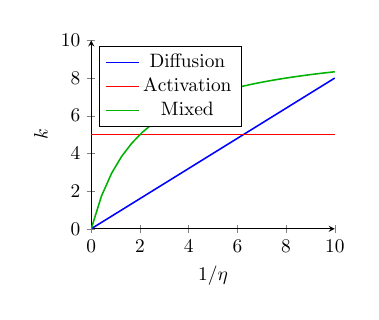
\begin{tikzpicture}[scale=0.7]
\begin{axis}[
    xlabel={$1/\eta$},
    ylabel={$k$},
    xmin=0, xmax=10,
    ymin=0, ymax=10,
    axis lines=left,
    width=6cm,
    height=5cm,
    legend pos=north west
]
\addplot[blue, thick, domain=0:10] {0.8*x};
\addlegendentry{Diffusion}

\addplot[red, thick, domain=0:10] {5};
\addlegendentry{Activation}

\addplot[green!70!black, thick, domain=0:10] {5*x/(1+0.5*x)};
\addlegendentry{Mixed}
\end{axis}
\end{tikzpicture}

\vspace{0.2cm}
\small Diffusion-controlled reactions slow down in viscous media
\end{columns}

\end{frame}

% ===========================================================================
% Slide: Material Balance Equation
% ===========================================================================
\begin{frame}{The Material Balance Equation}

\textbf{General equation for species J undergoing transport and reaction:}

\keyeq{\frac{\partial [J]}{\partial t} = D \frac{\partial^2 [J]}{\partial x^2} - v \frac{\partial [J]}{\partial x} - k_r [J]}

\vspace{0.3cm}

\textbf{Three contributions:}

\begin{enumerate}
\item \textbf{Diffusion:} $D \frac{\partial^2 [J]}{\partial x^2}$
\begin{itemize}
\item Spreading due to concentration gradients
\item Fick's second law
\item Always acts to smooth out concentration differences
\end{itemize}

\item \textbf{Convection:} $-v \frac{\partial [J]}{\partial x}$
\begin{itemize}
\item Bulk flow of fluid
\item $v$ = flow velocity
\item Important in stirred reactors, flowing systems
\end{itemize}

\item \textbf{Reaction:} $-k_r [J]$
\begin{itemize}
\item Chemical transformation
\item Acts as a sink (or source if production)
\item Local consumption
\end{itemize}
\end{enumerate}

\end{frame}

% ===========================================================================
% Slide: Diffusion-Reaction Coupling
% ===========================================================================
\begin{frame}{Coupled Diffusion and Reaction}

\textbf{Simplified 1D case (no convection):}

\[ \frac{\partial c}{\partial t} = D \frac{\partial^2 c}{\partial x^2} - kc \]

\vspace{0.2cm}

\textbf{Steady-state solution ($\partial c/\partial t = 0$):}

\[ D \frac{d^2 c}{dx^2} = kc \]

\textbf{General solution:}
\[ c(x) = A e^{-x/\lambda} + B e^{x/\lambda} \]

where the \textbf{reaction-diffusion length} is:

\keyeq{\lambda = \sqrt{\frac{D}{k}}}

\vspace{0.2cm}

\textbf{Physical Meaning:}
\begin{itemize}
\item $\lambda$: Typical distance a molecule diffuses before reacting
\item Large $\lambda$ (slow reaction): Penetrates far
\item Small $\lambda$ (fast reaction): Reacts near surface
\end{itemize}

\end{frame}

% ===========================================================================
% Slide: Example - Diffusion with Reaction
% ===========================================================================
\begin{frame}{Example: Iodine Diffusion in Starch Solution}

\textbf{Experiment:} I$_2$ vapor diffuses into aqueous starch solution where it reacts:

\[ \text{I}_2 + \text{starch} \to \text{blue complex} \]

\vspace{0.2cm}

\begin{columns}[T]
\column{0.55\textwidth}
\textbf{Observation:}
\begin{itemize}
\item Sharp blue front moves down column
\item Front position: $x_f \propto \sqrt{t}$
\item Width of colored region $\sim \lambda$
\end{itemize}

\vspace{0.2cm}
\textbf{Analysis:}

With $D = 2 \times 10^{-9}$ m$^2$ s$^{-1}$ and $k = 0.1$ s$^{-1}$:

\[ \lambda = \sqrt{\frac{D}{k}} = \sqrt{\frac{2 \times 10^{-9}}{0.1}} = 1.4 \times 10^{-4} \text{ m} = 0.14 \text{ mm} \]

Sharp front because fast reaction confines I$_2$ to thin layer.

\column{0.45\textwidth}
\centering
\textbf{Concentration Profile:}

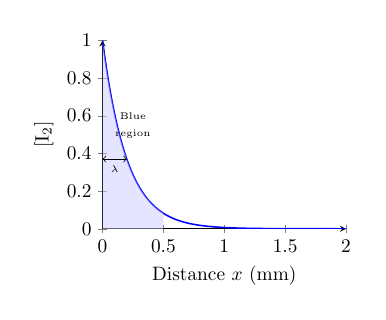
\begin{tikzpicture}[scale=0.7]
\begin{axis}[
    xlabel={Distance $x$ (mm)},
    ylabel={[I$_2$]},
    xmin=0, xmax=2,
    ymin=0, ymax=1,
    axis lines=left,
    width=6cm,
    height=5cm
]
\addplot[blue, thick, domain=0:2, samples=100] {exp(-5*x)};
\addplot[fill=blue!20, draw=none, opacity=0.5, domain=0:0.5, samples=50] {exp(-5*x)} \closedcycle;
\node at (axis cs:0.25,0.6) {\tiny Blue};
\node at (axis cs:0.25,0.5) {\tiny region};
\draw[<->] (axis cs:0,0.37) -- (axis cs:0.2,0.37) node[midway, below] {\tiny $\lambda$};
\end{axis}
\end{tikzpicture}
\end{columns}

\textbf{Application:} Pattern formation in biology (morphogen gradients), catalysis (porous catalysts)

\end{frame}

% ===========================================================================
% Slide: Damköhler Number
% ===========================================================================
\begin{frame}{The Damköhler Number}

\textbf{Dimensionless parameter comparing reaction and diffusion rates:}

\keyeq{\text{Da} = \frac{\text{reaction rate}}{\text{diffusion rate}} = \frac{kL^2}{D}}

where $L$ is characteristic length scale.

\vspace{0.3cm}

\textbf{Physical Interpretation:}

\begin{columns}[T]
\column{0.5\textwidth}
\textbf{Da $\ll$ 1:} Diffusion-limited
\begin{itemize}
\item Reaction is slow
\item Concentration uniform
\item Well-mixed approximation valid
\item Rate $\propto k$
\end{itemize}

\textbf{Da $\gg$ 1:} Mass-transfer limited
\begin{itemize}
\item Reaction is fast
\item Steep concentration gradients
\item Rate $\propto D/L$
\item Transport controls
\end{itemize}

\column{0.5\textwidth}
\centering
\textbf{Concentration Profiles:}

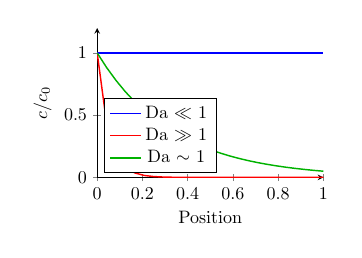
\begin{tikzpicture}[scale=0.65]
\begin{axis}[
    xlabel={Position},
    ylabel={$c/c_0$},
    xmin=0, xmax=1,
    ymin=0, ymax=1.2,
    axis lines=left,
    width=6cm,
    height=4.5cm,
    legend pos=south west
]
\addplot[blue, thick, domain=0:1] {1};
\addlegendentry{Da $\ll$ 1}

\addplot[red, thick, domain=0:1] {exp(-20*x)};
\addlegendentry{Da $\gg$ 1}

\addplot[green!70!black, thick, domain=0:1] {exp(-3*x)};
\addlegendentry{Da $\sim$ 1}
\end{axis}
\end{tikzpicture}
\end{columns}

\vspace{0.2cm}

\textbf{Applications:} Chemical reactors, catalysis, biological systems

\end{frame}

% ===========================================================================
% Slide: Worked Example 1
% ===========================================================================
\begin{frame}{Worked Example 1: Calculate $k_d$ for Specific Molecules}

\textbf{Problem:} Calculate the diffusion-controlled rate constant for the reaction between two identical molecules with $r = 0.5$ nm in water at 25°C.

\vspace{0.2cm}

\textbf{Given:}
\begin{itemize}
\item $r_A = r_B = 0.5$ nm = $5 \times 10^{-10}$ m
\item $T = 298$ K
\item $\eta_{water} = 8.9 \times 10^{-4}$ Pa$\cdot$s
\item $k_B = 1.381 \times 10^{-23}$ J K$^{-1}$
\item $N_A = 6.022 \times 10^{23}$ mol$^{-1}$
\end{itemize}

\vspace{0.2cm}

\textbf{Solution:}

\textbf{1. Contact distance:} $R^* = r_A + r_B = 1.0$ nm = $1.0 \times 10^{-9}$ m

\textbf{2. Diffusion coefficient for each molecule:}
\[ D = \frac{k_B T}{6\pi \eta r} = \frac{1.381 \times 10^{-23} \times 298}{6\pi \times 8.9 \times 10^{-4} \times 5 \times 10^{-10}} = 4.9 \times 10^{-10} \text{ m}^2\text{ s}^{-1} \]

\end{frame}

% ===========================================================================
% Slide: Worked Example 1 cont.
% ===========================================================================
\begin{frame}{Worked Example 1 (continued)}

\textbf{3. Combined diffusion coefficient:}
\[ D_{rel} = D_A + D_B = 2D = 9.8 \times 10^{-10} \text{ m}^2 \text{ s}^{-1} \]

\textbf{4. Smoluchowski rate constant:}
\[ k_d = 4\pi R^* D_{rel} N_A \]
\[ k_d = 4\pi \times 1.0 \times 10^{-9} \times 9.8 \times 10^{-10} \times 6.022 \times 10^{23} \]
\[ k_d = 7.4 \times 10^6 \text{ m}^3 \text{ mol}^{-1} \text{ s}^{-1} \]

\vspace{0.2cm}

\textbf{Convert to M$^{-1}$ s$^{-1}$:}
\[ k_d = 7.4 \times 10^9 \text{ M}^{-1} \text{ s}^{-1} \]

\vspace{0.3cm}

\emphbox{\textbf{Answer:} $k_d \approx 7 \times 10^9$ M$^{-1}$ s$^{-1}$ - close to universal diffusion limit!}

\end{frame}

% ===========================================================================
% Slide: Worked Example 2
% ===========================================================================
\begin{frame}{Worked Example 2: Determine Reaction Control Regime}

\textbf{Problem:} A reaction has $k_{obs} = 5 \times 10^8$ M$^{-1}$ s$^{-1}$ in water at 25°C. The activation energy is $E_a = 25$ kJ/mol. Is this reaction diffusion-controlled or activation-controlled?

\vspace{0.2cm}

\textbf{Solution:}

\textbf{1. Compare to diffusion limit:}
\[ k_d \approx 7 \times 10^9 \text{ M}^{-1} \text{ s}^{-1} \]
\[ \frac{k_{obs}}{k_d} = \frac{5 \times 10^8}{7 \times 10^9} \approx 0.07 = 7\% \]

The observed rate is only 7\% of diffusion limit.

\vspace{0.2cm}

\textbf{2. Check activation energy:}
\begin{itemize}
\item Diffusion-controlled: $E_a \sim 10-20$ kJ/mol
\item Observed: $E_a = 25$ kJ/mol (slightly higher)
\end{itemize}

\vspace{0.2cm}

\emphbox{\textbf{Conclusion:} Mixed control with significant activation barrier. Encounters are frequent, but not every encounter leads to reaction.}

\end{frame}

% ===========================================================================
% Slide: Summary
% ===========================================================================
\begin{frame}{Summary: Topic 18B}

\textbf{Key Concepts:}

\begin{enumerate}
\item \textbf{Cage Effect:} Multiple collisions within solvent cage
\begin{itemize}
\item Changes encounter dynamics vs gas phase
\item Effective single "encounter" event
\end{itemize}

\item \textbf{Two-Step Mechanism:} Diffusion + Activation
\begin{itemize}
\item $k_{eff}^{-1} = k_d^{-1} + (Kk_a)^{-1}$
\item Two resistances in series
\end{itemize}

\item \textbf{Smoluchowski Theory:} $k_d = 4\pi R^* D N_A \approx \frac{8RT}{3\eta}$
\begin{itemize}
\item Diffusion limit: $\sim 10^{10}$ M$^{-1}$ s$^{-1}$ in water
\item Depends on $T/\eta$, nearly size-independent
\end{itemize}

\item \textbf{Fick's Laws:} Foundation of diffusion theory
\begin{itemize}
\item First law: Flux proportional to gradient
\item Second law: Time evolution of concentration
\end{itemize}

\item \textbf{Material Balance:} Couples diffusion, convection, and reaction
\begin{itemize}
\item Reaction-diffusion length: $\lambda = \sqrt{D/k}$
\item Damköhler number: Da $= kL^2/D$
\end{itemize}
\end{enumerate}

\end{frame}

% ===========================================================================
% Slide: Practice Problems
% ===========================================================================
\begin{frame}{Practice Problems}

\textbf{Problem 1:} Calculate the diffusion coefficient of a spherical protein with radius 3.0 nm in water at 25°C ($\eta = 0.89$ mPa$\cdot$s).

\vspace{0.2cm}

\textbf{Problem 2:} For a reaction with $k_{obs} = 2 \times 10^9$ M$^{-1}$ s$^{-1}$ at 25°C, estimate what fraction of encounters lead to reaction. Assume $k_d = 7 \times 10^9$ M$^{-1}$ s$^{-1}$.

\vspace{0.2cm}

\textbf{Problem 3:} A reaction rate triples when temperature increases from 15°C to 35°C. The viscosity decreases by a factor of 1.8 over this range. Is the reaction diffusion-controlled or activation-controlled? Estimate $E_a$.

\vspace{0.2cm}

\textbf{Problem 4:} Calculate the reaction-diffusion length $\lambda$ for a first-order reaction with $k = 1.0$ s$^{-1}$ and $D = 10^{-9}$ m$^2$ s$^{-1}$.

\vspace{0.2cm}

\textit{Answers: (1) $D \approx 7.3 \times 10^{-11}$ m$^2$ s$^{-1}$; (2) $\sim$29\%; (3) Activation-controlled, $E_a \approx 35$ kJ/mol; (4) $\lambda \approx 30$ $\mu$m}

\end{frame}

% ===========================================================================
% Slide: Applications and Extensions
% ===========================================================================
\begin{frame}{Applications and Modern Extensions}

\textbf{Biological Systems:}
\begin{itemize}
\item Enzyme-substrate encounter ($k_{cat}/K_M$ often near diffusion limit)
\item Signal transduction cascades
\item Protein-protein interactions
\item Morphogen gradient formation
\end{itemize}

\vspace{0.2cm}

\textbf{Chemical Engineering:}
\begin{itemize}
\item Reactor design (stirring requirements)
\item Catalysis in porous media
\item Gas-liquid reactions
\item Fast reactions in flow systems
\end{itemize}

\vspace{0.2cm}

\textbf{Modern Developments:}
\begin{itemize}
\item Single-molecule tracking (fluorescence microscopy)
\item Microfluidics and confinement effects
\item Anomalous diffusion in crowded environments
\item Brownian dynamics simulations
\end{itemize}

\vspace{0.2cm}

\emphbox{Next: Transition-State Theory provides molecular details of the activation barrier}

\end{frame}

% ===========================================================================
% Slide: Interactive Resources for Topic 18B
% ===========================================================================
\begin{frame}{Interactive Learning: Topic 18B}

\begin{columns}[c]
\column{0.65\textwidth}
\textbf{Explore Diffusion-Controlled Reactions Interactively!}

\vspace{0.3cm}

\textbf{Interactive Jupyter Notebook Features:}
\begin{itemize}
    \item \textbf{Cage Effect Simulator}: Visualize solvent cage dynamics
    \item \textbf{Smoluchowski Calculator}: Compute diffusion-controlled rates
    \item \textbf{Encounter Pair Dynamics}: Animated trajectories
    \item \textbf{Viscosity Effects}: Interactive rate vs $\eta$ plots
    \item \textbf{Activation vs Diffusion}: Regime comparison
    \item \textbf{Real Examples}: Radical recombination, enzyme kinetics
\end{itemize}

\vspace{0.3cm}

\textbf{Notebook:} \texttt{02\_Diffusion\_Controlled.ipynb}

\column{0.35\textwidth}
\centering
\textbf{Scan to Open:}

\vspace{0.3cm}

\includegraphics[width=0.8\textwidth]{QR_codes/02_Diffusion_Controlled.png}

\vspace{0.3cm}

{\footnotesize Or navigate to:\\
\texttt{Reaction\_Dynamics\_Interactive/}}

\end{columns}

\end{frame}
